\subsubsection{Modelling Language Context Free Grammar}
Using the Extended Backus-Naur Formalism for defining context free grammars, we translate the concrete syntax of our feature and configuration into an abstract syntax tree. From both abstract syntax trees in figure \ref{ast-feature} and figure \ref{ast-config},  we are able to inductively deduce the finite set of terminal and non-terminal symbols, that are required to implement our novel variability management technique.

\begin{figure}[H]
\caption{Abstract Syntax Tree for a Feature}
\centering
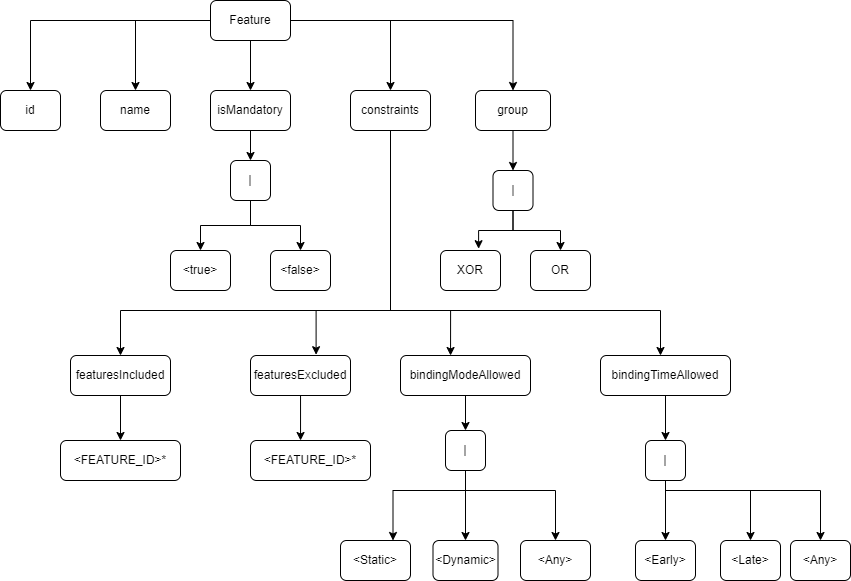
\includegraphics[width=0.5\textwidth]{diagrams/ast-feature.png}
\label{ast-feature}
\end{figure}

\begin{figure}[H]
\caption{Abstract Syntax Tree for a Feature Configuration}
\centering
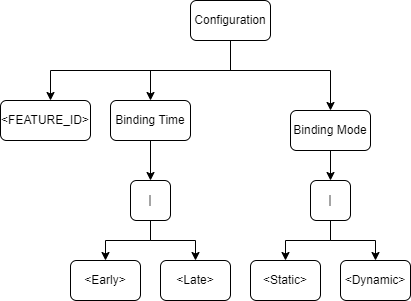
\includegraphics[width=0.3\textwidth]{diagrams/ast-conf.png}
\label{ast-config}
\end{figure}

-----------------------------------------------------------------------------------
\begin{verbatim}
machine "DSL FSM" [
	S0 = precompile time
	S1 = command ready
	S2 = compile time
	S3 = run time
	
	initial precompile time
	
	state precompile time[
	    on input "create_product" 
	        output "success" and go to S1
		on input "create_product" 
		    output "error" and go to S1
		on input "console_load_product PRODUCT_NAME" 
		    output "success" and go to S1
		on input "ls" output "PL list" and go to S1
		on input "man ALL/COMMAND" 
		    output "documentation" and go to S1
		on input "show ALL/FEATURE_ID" 
		    output "feature model" and go to S1
		on input "exit" go to S0
	]
	
	state command ready[
		on input "validate_config" 
		    output "bindingViolations" and go to S1
		on input "validate_config"
		    output "success" and go to S2
	]
	
	state compile time[
		on input "run_config" 
		    output "success" and go to S3
		on input "run_config" 
		    output "error" and go to S2
	]
	
	state run time[
		on input "load FEATURE_ID" 
		    output "sucess" and go to S3
		on input "load FEATURE_ID" 
		    output "error" and go to S3
		on input "unload FEATURE_ID" 
		    output "sucess" and go to S3
		on input "unload FEATURE_ID" 
		    output "error" and go to S3
	]
]
\end{verbatim}

\begin{figure}[H]
\caption{DSL Grammar Finite State Machine}
\centering
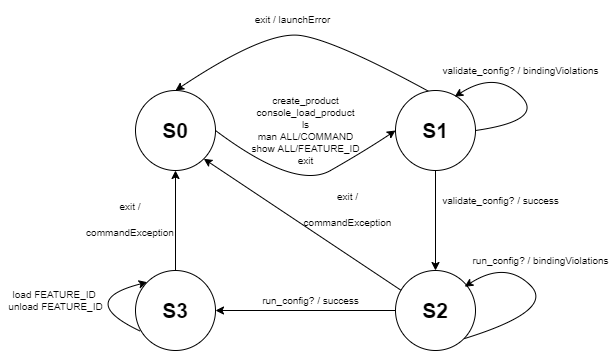
\includegraphics[width=0.5\textwidth]{diagrams/fsm.png}
\label{fsm}
\end{figure}

\textbf{DSL Lexical and Syntactic Structure: }Overall, our internal domain specific language to manage variability has four distinct states i.e. pre-compile, command ready, compile time and run time. As shown in figure \ref{fsm} above, each state possesses a set of transitions that are triggered by user actions in the form of command executions. In the pre-compile state, a product line can be instantiated and loaded, product line instance properties can be configured, binding properties can be assigned and overall feature constraints can be set. The command ready state focuses on validating user defined configurations based on rules and constraints that have been set. A compile time state is characterised by running validated configurations. Finally, at runtime, a configuration can be adapted based on the implications of its time and mode bindings as well as the interactive effect of each feature binding. It is also important to note that there is the likelihood of each state transitioning into the initial state either through an exit operation or an illegal operation that throws an exception.
--------------------------------------------------------------------------

\subsubsection{Modelling Language Context Free Grammar}
Using the Extended Backus-Naur Formalism for defining context free grammars, we translate the concrete syntax of our feature and configuration into an abstract syntax tree. From both abstract syntax trees in figure \ref{ast-feature} and figure \ref{ast-config},  we are able to inductively deduce the finite set of terminal and non-terminal symbols, that are required to implement our novel variability management technique.

\subsubsection{Context Free Grammar Production Rules}
-------------------------------------------------------------------------------
\subsubsection{Concrete Textual Syntax: }The fundamental building blocks of feature models are features. In our language, feature instances of robotic product lines are represented as JSON objects. Every feature instance is decoupled to separate configurable attributes from no-configurable ones. Configurable attributes provide users with the capability to adapt features based on a feature's assigned binding time and binding mode attributes. For a given feature instance, end users also have the capability to set constraints on features. In the sample code snippets provided below, we present the valid syntax that defines the capabilities of feature instantiation.

Our technique for managing variability makes use of a feature's binding time and binding mode attributes, to dynamically adapt an instance of a robotic model to fit varying usage contexts. For this reason, binding time and binding mode feature attributes are decoupled from the main set of feature attributes, mainly to separate concerns which in tun reduces the complexity of implementing variation points in user defined models. The decoupled feature attributes are represented as an \textbf{id} referenced object in a configuration file. In the code snippet below, we provide an illustration of the concrete syntax of a feature present in a configuration.

\begin{listing}
\begin{minted}{json}
{
    "id": "oocje_root",
    "props": {
        "mode": "Static",
        "time": "Early",
    }
}
\end{minted}
\caption{JSON example} 
\label{json-example}
\end{listing}
-------------------------------------------------------------------------------
---------------------------------------------------------------------------------------------------------------------------------------------------------------

\subsubsection{Concrete Syntax Overview}
The concrete syntax of our language can be expressed graphically and textually through feature models. The key selling point of our implementation is to give users of the capability to create their own custom programs that will be in the form of robotic feature models. In that, end users of our domain specific language will be able to implement their own feature models of example robots that are adaptable in varying contexts.
\subsubsection{Concrete Graphical Syntax}
Figure \ref{simplebot} shows the concrete graphical syntax of our language. Graphically, our language can be represented as a feature model. Feature models are optimum because they are a standardised means of capturing relevant concrete information about features in our \textit{simpleBot} example as well as show the hierarchical dependencies that exist between modelled features. 

\begin{figure}[H]
\caption{SimpleBot Modelled in FeatureIDE}
\centering
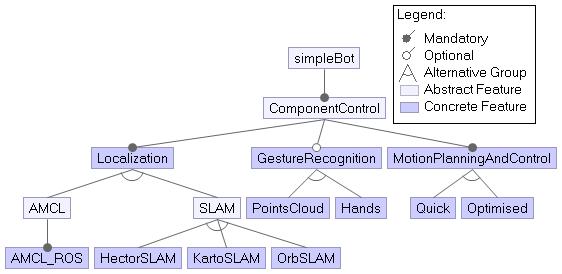
\includegraphics[width=0.5\textwidth]{diagrams/simpleBot.png}
\label{simplebot}
\end{figure}
\subsubsection{Concrete Textual Syntax: }
Textually, custom models of robots created by end users can be represented as a string of nested objects. In each feature object, feature attributes defined as key value pairs. These attributes can be used to either describe a feature or constrain it. In our implementation, feature bindings are separated from other feature attributes in an attempt to separate concerns. The snippet in listing \ref{feat-conc-text} shows the textual model of a subsection of the feature model shown in figure \ref{simplebot}.


\begin{listing}
\caption{Textual Sample of Features}
\begin{minted}[
framesep=2mm,
baselinestretch=1.2,
bgcolor=LightGray,
fontsize=\footnotesize
]{Json}
{
    "id": "root_feature",
    "name": "simpleBot",
    "group": "",
    "isMandatory": true,
    "sub": [
        {
        "id": "F0",
        "name": "ComponentControl",
        "constraints": {
        "featuresIncluded": [],
        "featuresExcluded": [],
        "bindingTimeAllowed":"Early",
        "bindingModeAllowed":"Static"
        },
        "group": "OR",
        "isMandatory": true
        "sub":[
            {
            "id": "F1",
            "name": "Localization",
            "constraints": {
            "featuresIncluded": [],
            "featuresExcluded": [],
            "bindingTimeAllowed":"Early",
            "bindingModeAllowed":"Static"
            },
            "group": "",
            "isMandatory": true
            }]}]}
\end{minted}
\label{feat-conc-text}
\end{listing}

Features  present in a feature model specification posses binding time and binding mode attributes which are used by our language to manage variability in modelled robotic systems. As mentioned earlier, in our architectural design, binding attributes are separated from the main feature model for the sole purpose of separating configurable attributes from no-configurable ones. Listing
\ref{bind-conc-text} captures the concrete textual syntax of feature binding attributes / properties. 
\begin{listing}
\caption{Textual Sample of Feature Bindings}
\begin{minted}[
framesep=2mm,
baselinestretch=1.2,
bgcolor=LightGray,
fontsize=\footnotesize
]{Json}
{
"properties": [
    {
    "id": "F0",
    "props": {
        "mode": "Static",
        "time": "Early"
    }
    },
    {
    "id": "F1",
    "props": {
        "mode": "Static",
        "time": "Early"
    }
]
}
\end{minted}
\label{bind-conc-text}
\end{listing}

\begin{table}[htbp]
\caption{Language Tokens}
Lexically our language possesses a number of legal tokens. Tokens can be identified and extracted from the attributes that make up a feature in a feature model. Table \ref{tab:langlex} shows all identified tokens together with their corresponding regular expressions that define their legal or valid lexical structures.
\begin{center}
\begin{tabular}{|c|c|}
\hline
    Token & Regular Expression \\\hline
                             id & $\{(a-zA-Z-0-9)^+\}$  \\\hline
                             name & $\{(a-zA-Z)^+\}$ \\ \hline
                             featuresIncluded & $\{(a-zA-Z-0-9 | a-zA-Z-0-9)^+\}$  \\ \hline
                             featuresExcluded & $\{(a-zA-Z-0-9 | a-zA-Z-0-9)^+\}$\\ \hline
                             bindingTimeAllowed & $\{(Early | Late | Any)\}$\\ \hline
                             bindingModeAllowed & $\{(Static | Dynamic | Any)\}$\\\hline
                             group & $\{("" | OR | XOR)\}$\\ \hline
                             isMandatory & $\{[(true | false)]\}$\\ \hline
                             sub & $\{[({(a-zA-Z):(a-zA-Z)}^+,)]\}$\ \\ \hline
                             time & $\{(Early | Late)\}$\\ \hline
                             mode & $\{(Static | Dynamic)\}$\\ \hline
\end{tabular}
\label{tab:langlex}
\end{center}
\end{table}

For each identified token in our language, we translate a valid expression of it into regular expressions to demonstrate which valid forms of these token can exist in our language. Syntactically, features and their bindings model attributes as key value pairs wrapped in an object.

\subsubsection{Syntactic Structure}
\begin{itemize}
    \item[] \textbf{Develop Mock-up Examples: }Our language can be used to develop mock up examples that demonstrate the language's expressiveness. In the context of our study, examples refer to modelled features of robot product lines. Figure \ref{ex1} and \ref{ex2} graphically show feature models of example systems i.e. service robots. Each feature present in a model can be expressed textually in terms of our language as shown in \ref{feat-conc-text} and \ref{bind-conc-text}. Inspiration for these examples were drawn from general utilities robots and disinfection robots such as TIAGo and UVD Model C.
    
    \begin{figure}[H]
    \caption{Modelled Example One}
    \centering
    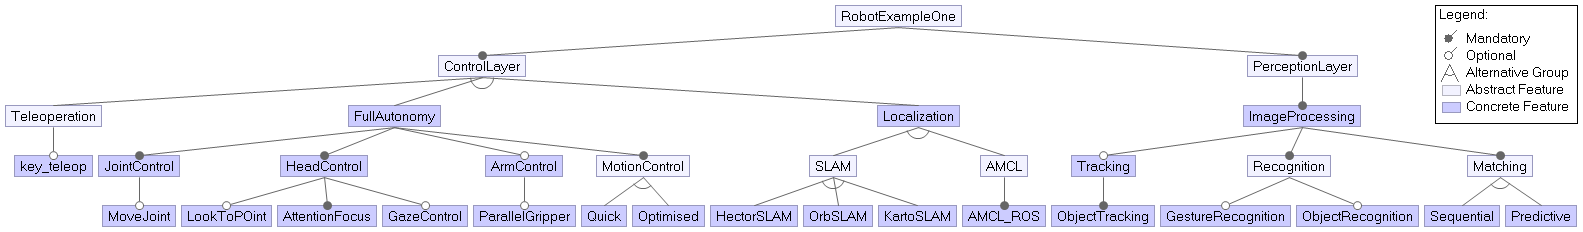
\includegraphics[width=\columnwidth]{diagrams/ex1.png}
    \label{ex1}
    \end{figure}
    
    \begin{figure}[H]
    \caption{Modelled Example Two}
    \centering
    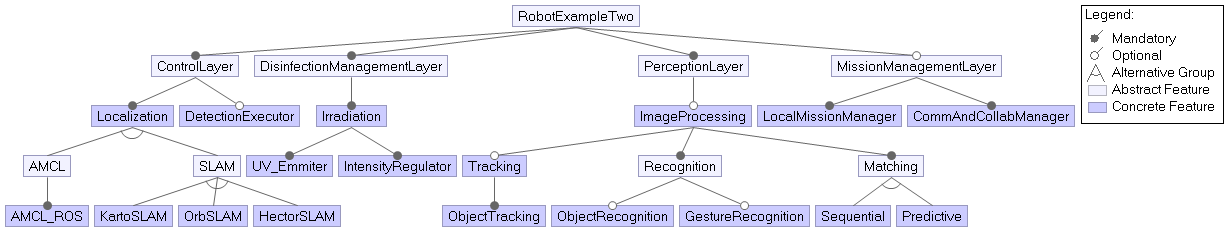
\includegraphics[width=\columnwidth]{diagrams/ex2.png}
    \label{ex2}
    \end{figure}
    
    In a model refinement step, that seeks to extend our mock-up examples against our requirements, we analyse requirements associated with our language, justify if these requirements are met and then proceed to provide examples or evidence of these requirements that have been met.
    
    \item[] \textbf{Specify Terminals: }
    \item[] \textbf{Identify Syntactic Categories: }
    \item[] \textbf{Specify Grammar Rules: }
\end{itemize}
---------------------------------------------------------------------------
Terminals
\begin{table}[htbp]
\caption{Language Tokens}
\begin{center}
\begin{tabular}{|c|c|}
\hline
    Token & Regular Expression \\\hline
                             id & $\{(a-zA-Z-0-9)^+\}$  \\\hline
                             name & $\{(a-zA-Z)^+\}$ \\ \hline
                             featuresIncluded & $\{(a-zA-Z-0-9 | a-zA-Z-0-9)^+\}$  \\ \hline
                             featuresExcluded & $\{(a-zA-Z-0-9 | a-zA-Z-0-9)^+\}$\\ \hline
                             bindingTimeAllowed & $\{(Early | Late | Any)\}$\\ \hline
                             bindingModeAllowed & $\{(Static | Dynamic | Any)\}$\\\hline
                             group & $\{("" | OR | XOR)\}$\\ \hline
                             isMandatory & $\{[(true | false)]\}$\\ \hline
                             sub & $\{[({(a-zA-Z):(a-zA-Z)}^+,)]\}$\ \\ \hline
                             props & $\{({(a-zA-Z):(a-zA-Z)}^+,)\}$\ \\ \hline
                             time & $\{(Early | Late)\}$\\ \hline
                             mode & $\{(Static | Dynamic)\}$\\ \hline
\end{tabular}
\label{tab:langlex}
\end{center}
\end{table}
------------------------------------------------------------------------------
intro excess
------------------------------------------------------------------------------
The ISO/IEC/IEEE 42010\foot{https://www.iso.org/standard/50508.html} is a standard for architecture description of software systems that represents architecture as an aggregated or high-level view of software in terms of computational elements and connectors that enable interconnections between components. Architectural components as computational elements represent an abstraction of executable code and communicate with each other via connectors \cite{ref-arch}.

Architecturally, robotic systems are often built with a layered approach where each layer encapsulates a specific functionality and depends on the layer(s) above and below to complete a system's functionality \cite{soft-arch-robo}. As a frame of reference, robotic systems are made up of a control layer and an application layer. The control layer is essentially made up of drivers that communicate directly with hardware components and an application layer utilizes the drivers in the control layer to perform a specified set of tasks.



For that matter, the decision to determine valid feature configurations based on features'  binding time and mode can be tricky and somehow cumbersome. Thus, there needs to be an optimum mechanism for doing this for efficient performance results. To derive configurations effectively, the dependencies and constraints that exist between features must be well established.
In doing so, the most significant problem we have identified lies in the re-configuration of robotic systems with respect to variability. SERA and architectures similar to it do not possess this functionality. These robotic architectures do not provide roboticists with the means and techniques required to manage variability effectively. Thus, there is the need to provide techniques and guidelines to do so in the form of a framework.

The semantics of such a framework with binding time and binding mode can be quite complex, since valid (re-)configurations are not only constrained by dependencies among features, but also by valid/invalid combinations of the binding time and binding mode of dependent features. For instance, a feature cannot be bound statically when it is dependent on a dynamic feature, since the latter can be activated or deactivated at any time. When a scenario like this is not handled properly, there is the tendency of ending up in an unspecified system state or a system crash.


: & ':' & Colon\\ \hline
[ & '[' & ListOpen\\ \hline
] & ']' & ListClose\\ \hline
\{ & '\{' & DictOpen\\ \hline
\} & '\}' & DictClose\\ \hline
============================================================================
\subsubsection{Mechanisms That Realise Static and Dynamic Binding}
Realising static and dynamic binding in robotic applications can be tricky due to programming language compatibility and limitations. For both static and dynamic binding, there are both C++ and Python mechanisms that can be used to realise them as shown in Table \ref{tab:realmecha}. However, integrating both the C++ preprocessor and ROS pluginlib into our implementation was not feasible due to language compatibility issues. Thus, to realise static binding, we used roslaunch to bind feature nodes through a launch file. Dynamically, we initialised parameters on the ROS parameter server to keep track of bound robotic features and binding time states. To realise binding time (i.e. Early and Late), we used ROS parameters and roslaunch to set and update server parameters as markers for determining configuration execution states. Early or compile time consists of the time period before the configuration is run to the point where the run sequence begins. After running the configuration, binding time switches to Late. Thus, at compile time, a ROS parameter is set to \textit{early} through a ROS launch argument to mark early binding time. Immediately a configuration is run, the same ROS parameter is re-initialised to \textit{late} indicated runtime.

\begin{table}[htbp]
\caption{Static and Dynamic Binding Mechanisms}
\begin{center}
\begin{tabular}{|c|c|}
\hline
    Binding & Mechanisms  \\ \hline
    Static & C preprocessor, antenna, rosrun, roslaunch \\ \hline
    Dynamic &  ROS pluginlib, ROS parameters  \\ \hline
    Early &  roslaunch, ROS parameters  \\ \hline
    Late &  ROS parameters  \\ \hline
\end{tabular}
\label{tab:realmecha}
\end{center}
\end{table}